
% Pressure-scope revision: analyses/021-2026-09-10-training-results-figures/pressure-scope/observations/O016-pressure-placement.md; evidence.py, figures.py, tables.py.
% Source observation: analyses/018-2026-09-08-results-materials/observations/O012-manuscript-results.md
% Argument revision after adversarial review, 2026-09-05. Hand-edited.
% Sources and claim boundaries: positioning.md and reviews/2026-09-05-adversarial/.
% Result preview authorized 8 September 2026; evidence: Analysis 018 O002/O003/O007/O011.
\section{Introduction}
\label{sec:introduction}

Activation sparsity can improve transformer inference efficiency when specialized kernels can skip computation and memory accesses of zero activations. Recently, \citet{cetin2026sparser} has succesfully demonstrated inference speedups from train-time pressure and specialized kernel design. This result motivates a follow-up question: \emph{how broadly and aggressively should train-time interventions be applied throughout the transformer to induce exploitable sparsity while reducing latency at an acceptable quality cost?}

Existing approaches differ in where and how they induce sparsity. TEAL applies post-hoc, training-free thresholding to pretrained models; ProSparse and \citet{cetin2026sparser} apply $\ell_1$ regularization to feed-forward (FFN) activations during training; and Q-Sparse applies top-$k$ sparsification to both FFN and attention activations~\citep{liu2024teal,song2024prosparse,wang2024qsparse}. However, these studies do not isolate the effects of different train-time sparsity interventions under a common training protocol. Under matched pretraining conditions using models from the Pythia family~\citep{biderman2023pythia}, we systematically vary the coverage and intensity of train-time sparsity interventions accros activation sites and measure their model-wide sparsity ($\Smodel$), and execution efficiency.

% Source: analyses/033-2026-09-21-14m-latency-quality-frontier/02_three_panel.py
% Observation: analyses/033-2026-09-21-14m-latency-quality-frontier/observations/005-three-panel.md
\begin{figure}[!t]
\centering
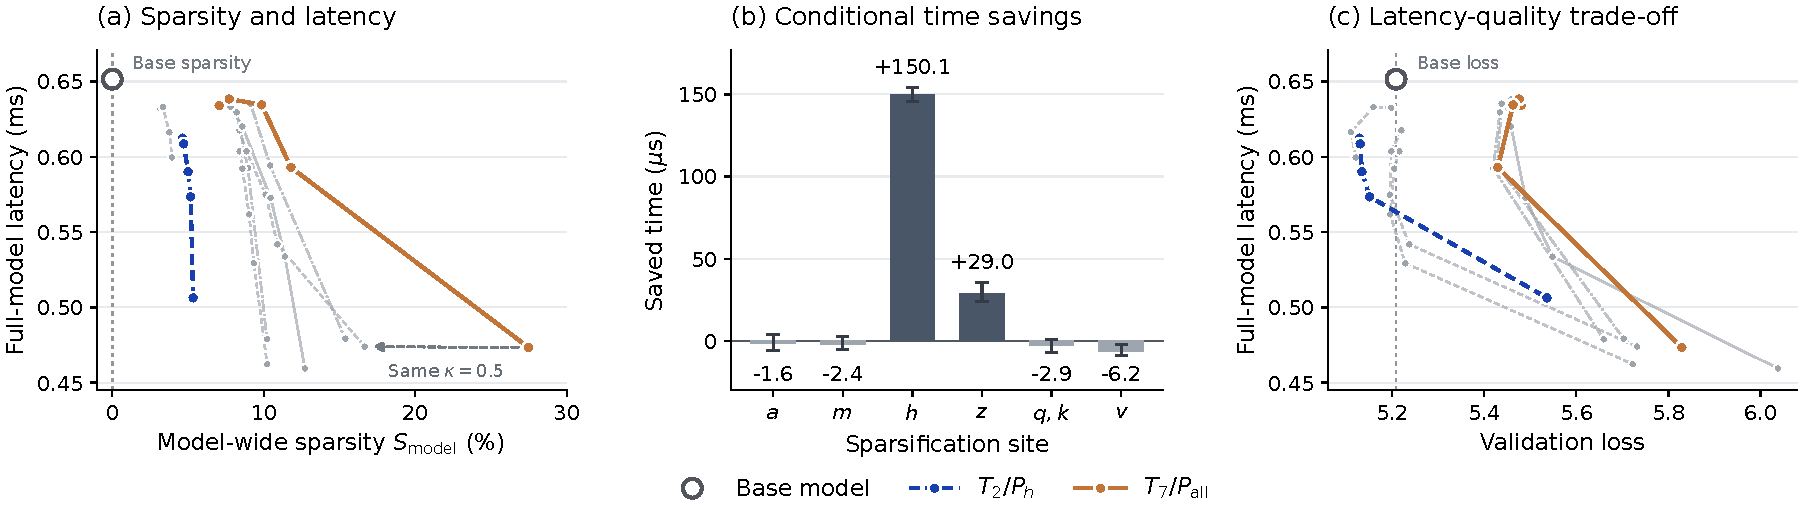
\includegraphics[width=\linewidth]{figures/04-14m-quality-savings-sparsity.pdf}
\caption{\textbf{Sparsity, execution savings and quality on Pythia-14M.}
\textbf{(a)} Model-wide logical sparsity $\Smodel$ versus full-model latency. The arrow connects $T_7/P_{\mathrm{all}}$ to $T_7/P_h$ at $\kappa=0.5$: 27.48\% and 16.66\% sparsity yield similar latency.
\textbf{(b)} Conditional execution ablations on $T_7/P_{\mathrm{all}}$ at $\kappa=0.5$ identify $h,z$ as the profitable skipping sites. Saved time is latency with one skipping path disabled minus latency with all paths enabled.
\textbf{(c)} Validation loss versus latency exposes the quality cost of broader sparsification.
Panels (a,c) show the same 40 checkpoints: $T_2/P_h$ is blue, $T_7/P_{\mathrm{all}}$ orange, and other recipes gray. Hollow markers and vertical guides denote base dense model; lines connect settings within recipes. Timings use BF16 on an RTX~5090, batch one and 2,048 tokens.
}
\label{fig:quality-sparsity-overview}
\end{figure}

We define an intervention by the placement of pressure ($P$) and thresholding ($T$). To keep the intervention space tractable, for $P$ we introduce Adam-orthogonalized $\ell_1$ activation pressure (OL1), limiting conflict with the task update while avoiding an additional pressure-strength sweep. For $T$ we use a fixed-threshold nonlinearity with $\kappa \in \{0, 0.01, 0.05, 0.1, 0.5\}$. The $P$ and $T$ placements are independent, so a recipe such as $T_7/P_{all}$ specifies their respective site sets, while sweeping $\kappa$ controls sparsification aggressiveness and traces the recipe's trade-off curve. Each model is then connected with an specialized kernel that connects its sparsity directly with execution benefit.

Under extensive 14M ablations, we first observe that broader intervention coverage can substantially extend attainable model-wide sparsity without translating into lower latency. At $\kappa=0.5$, expanding pressure and thresholding from four to seven sites more than doubles model-wide sparsity, from $12.71\%$ to $27.48\%$, while latency slightly increases from $0.459$ to $0.473$ ms (Fig.~\ref{fig:quality-sparsity-overview}(a)). Conditional kernel ablations then identify \(h\) and \(z\) as the profitable latency skipping paths, with the largest benefit at \(h\) (Fig.~\ref{fig:quality-sparsity-overview}(b)). Sparsity measurements reveal a related nonlocal effect: applying pressure only at \(h\) also increases sparsity at the thresholded \(z\) site, despite \(z\) receiving no direct pressure (Fig.~\ref{fig:pressure-layer-sparsity}). We call this effect \emph{sparsity spillover}. OL1 adds an additional geometry evidence for \(h\): applying pressure beyond \(h\) increases both the pressure-update norm and the component removed by orthogonalization, with the strongest effect at \(q,k,v\), indicating that these sites are less succeptible to sparsification (Fig.~\ref{fig:ol1-geometry}).

% Scale extension: analyses/038-2026-09-24-base-t2-t7-scale-frontier/observations/003-manuscript-integration.md; 04_manuscript_evidence.py.
Together, these ablations point to \(h\) and \(z\) as the most useful sparsification sites. They are more responsive to intervention and their sparsity translates into latency reduction, even when model-wide sparsity is smaller than broader recipes. This motivates a targeted \(T_2/P_h\) intervention: apply pressure only at \(h\), exploit its spillover to \(z\), and threshold only \(h\) and \(z\). At 14M and \(\kappa \leq 0.1\), \(T_2/P_h\) achieves both lower validation loss than the dense control and lower full-model latency (\(0.573\) vs. \(0.655\) ms, Fig.~\ref{fig:quality-sparsity-overview}(c)). We further compare $T_2/P_h$ and $T_7/P_h$ at 31M and 70M to test whether narrowing threshold coverage remains favorable while holding pressure placement fixed at $h$. The combinatorial space of train-time interventions and kernel designs motivates inverting the design problem: first specify the structure the kernel can exploit, then design train-time interventions to induce it.


% This convergence motivates a targeted recipe, \(T_2/P_h\): apply pressure only at \(h\), exploiting its spillover to \(z\), and restrict thresholding to \(h,z\). At 14M and \(\kappa=0.1\), this recipe achieves lower validation loss than the dense control and lower full-model latency (\(0.573\) versus \(0.655\) ms). A separate, same-checkpoint comparison isolates the contribution of sparse execution: enabling \(h,z\) skipping reduces latency by \(12.9\%\) relative to the same implementation with both paths disabled. At 70M, the targeted recipe retains its validation-loss advantage over the broader tested recipes, but its favorable low-loss latency result does not transfer directly. Together, these results support selecting sparsification sites through both their response to training interventions and their measured execution value.

% Two complementary diagnostics identify where susceptibility to sparsification and execution benefit coincide. 

% Two complementary diagnostics identify where susceptibility to sparsification and execution benefit coincide: the FFN hidden activation \(h\) and the input \(z\) to the attention-output projection. Applying pressure only at \(h\) increases sparsity at both sites relative to thresholding alone, although \(z\) receives no direct pressure. We call this nonlocal response sparsity spillover: an intervention confined to the FFN also increases sparsity in the thresholded attention branch. A separate execution decomposition converges on the same sites. With weights, thresholds, and other execution paths fixed, conditional kernel ablations identify \(h,z\) as the profitable skipping paths, with the largest benefit at \(h\), despite substantial arithmetic bypass elsewhere.


% %Activation sparsity can improve language-model inference efficiency when specialized kernels skip computations associated with zero activations. Recent work has shown that sparsity can be exposed in pretrained models through post-hoc clipping or induced during training, in both cases with measured inference speedups~\citep{liu2024teal,cetin2026sparser}. These results raise a practical design question: \emph{how to effectively sparsify a dense model in activations into an exploitable structure for optimized inference?}

% % Activation sparsity can improve transformer inference efficiency only when activations are exactly zero and those zeros occur in structures that the execution kernel can skip profitably~\citep{liu2024teal,cetin2026sparser}. 
% Activation sparsity can improve transformer inference efficiency under two necessary conditions: activations must be exactly zero, and the zeros must occur in structures that the execution kernel can skip profitably~\citep{cetin2026sparser}. The sparse structure can be induced in several ways. Training-time activation pressure adds a gradient component to induce smaller activation magnitudes, and thresholding maps small values into exact zeros. This creates two distinct design choices: (1) where to apply the pressure ($P$), and (2) where to threshold ($T$). Because a transformer block exposes several candidate activation sites, this placement problem is combinatorial by design. The central question is therefore \emph{where should pressure and thresholding be applied so that the resulting sparsity reduces inference latency at an acceptable quality cost?}

%two distinct design choices: where to apply training pressure ($P$) to induce smaller activations, and where to threshold ($T$) them to exact zeros. The central question is how these choices produce sparsity that kernels can exploit to reduce latency at an acceptable quality cost.

% Existing approaches make different choices about how and where to introduce sparsity. TEAL applies post-hoc training-free thresholding to pretrained models, ProSparse and \citet{cetin2026sparser} uses $\ell_1$ pressure on feed-forward (FFN) activations during training, and Q-Sparse applies top-$k$ sparsification to both FFN and attention activations ~\citep{liu2024teal,song2024prosparse,wang2024qsparse}. However, their results do not isolate the consequences of changing the train-time sparse intervention coverage and intensity under a common training protocol. We study these choices under matched pretraining conditions, connecting them with local and model-wide sparsity ($\Smodel$), measuring per-architecture and intervention maximum attainable sparsity ceiling ($\Smax$), and execution benefits.

%We study these factors under matched pretraining conditions, relating them to local and model-wide sparsity ($\Smodel$), characterizing the maximum attainable sparsity for each architecture and intervention ($\Smax$), and measuring the resulting execution benefits.


% % Source: analyses/033-2026-09-21-14m-latency-quality-frontier/02_three_panel.py
% % Observation: analyses/033-2026-09-21-14m-latency-quality-frontier/observations/005-three-panel.md
% \begin{figure}[!t]
% \centering
% 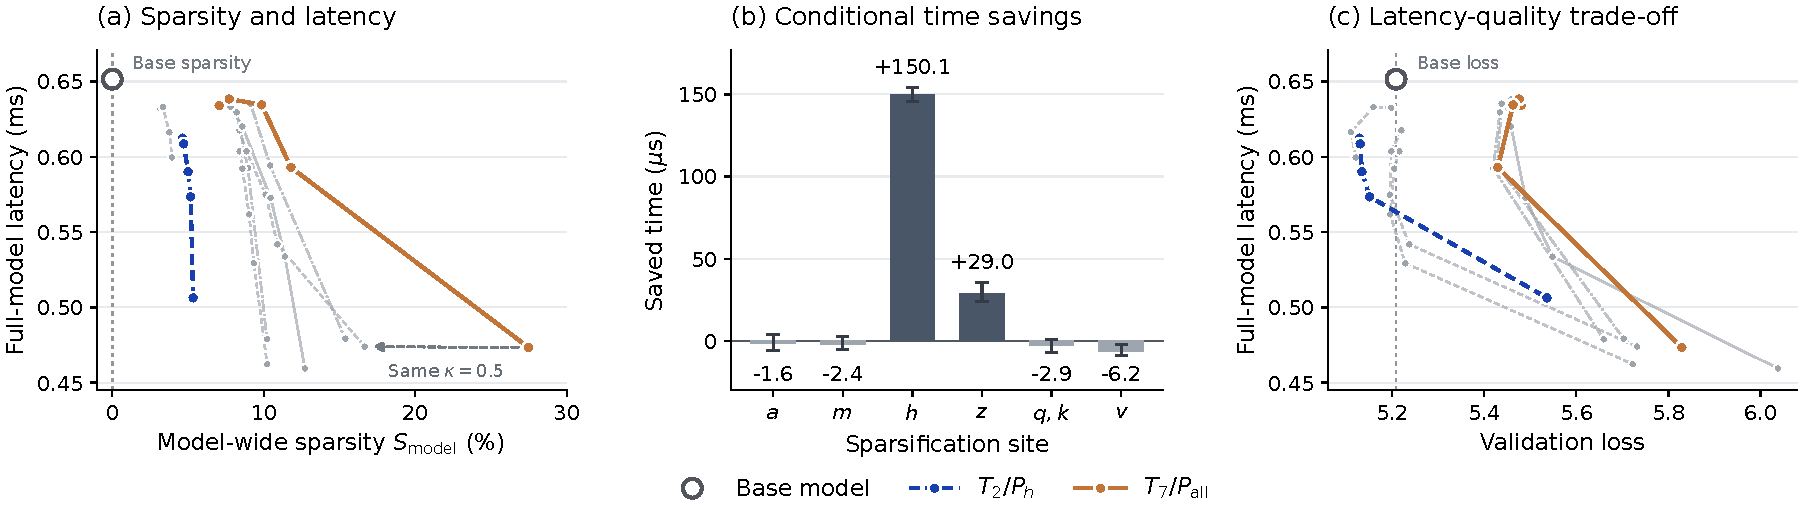
\includegraphics[width=\linewidth]{figures/04-14m-quality-savings-sparsity.pdf}
% \caption{\textbf{Sparsity, execution savings and quality on Pythia-14M.}
% \textbf{(a)} Model-wide logical sparsity $\Smodel$ versus full-model latency. The arrow connects $T_7/P_{\mathrm{all}}$ to $T_7/P_h$ at $\kappa=0.5$: 27.48\% and 16.66\% sparsity yield similar latency.
% \textbf{(b)} Conditional execution ablations on $T_7/P_{\mathrm{all}}$ at $\kappa=0.5$ identify $h,z$ as the profitable skipping sites. Saved time is latency with one skipping path disabled minus latency with all paths enabled, holding the checkpoint and thresholding fixed. Whiskers span differences between process means, not confidence intervals; these savings are not additive.
% \textbf{(c)} Validation loss versus latency exposes the quality cost of broader sparsification.
% Panels (a,c) show the same 40 checkpoints: $T_2/P_h$ is blue, $T_7/P_{\mathrm{all}}$ orange, and other recipes gray. Hollow markers and vertical guides denote Base; lines connect settings within recipes. Timings use BF16 on an RTX~5090, batch one and 2,048 tokens; panel (b) uses a separate controlled session.
% }
% \label{fig:quality-sparsity-overview}
% \end{figure}



% Our matched Pythia-14M~\citep{biderman2023pythia} experiments show that broader sparsification can increase model-wide sparsity without reducing latency. At aggressive thresholding (\(\kappa=0.5\)), extending thresholding and pressure from four sites to seven more than doubles model-wide sparsity, from \(12.71\%\) to \(27.48\%\), yet slightly increases latency, from \(0.459\) to \(0.473\) ms. Thus, aggregate sparsity alone does not determine execution benefit: evaluating an intervention requires identifying where its zeros emerge and which operations can exploit them profitably.

% Two complementary diagnostics identify where susceptibility to sparsification and execution benefit coincide: the FFN hidden activation \(h\) and the input \(z\) to the attention-output projection. Applying pressure only at \(h\) increases sparsity at both sites relative to thresholding alone, although \(z\) receives no direct pressure. We call this nonlocal response sparsity spillover: an intervention confined to the FFN also increases sparsity in the thresholded attention branch. A separate execution decomposition converges on the same sites. With weights, thresholds, and other execution paths fixed, conditional kernel ablations identify \(h,z\) as the profitable skipping paths, with the largest benefit at \(h\), despite substantial arithmetic bypass elsewhere.

% This convergence motivates a targeted recipe, \(T_2/P_h\): apply pressure only at \(h\), exploiting its spillover to \(z\), and restrict thresholding to \(h,z\). At 14M and \(\kappa=0.1\), this recipe achieves lower validation loss than the dense control and lower full-model latency (\(0.573\) versus \(0.655\) ms). A separate, same-checkpoint comparison isolates the contribution of sparse execution: enabling \(h,z\) skipping reduces latency by \(12.9\%\) relative to the same implementation with both paths disabled. At 70M, the targeted recipe retains its validation-loss advantage over the broader tested recipes, but its favorable low-loss latency result does not transfer directly. Together, these results support selecting sparsification sites through both their response to training interventions and their measured execution value.


% %-----
% Activation sparsity can improve language-model inference efficiency when specialized kernels skip computations associated with zero activations. Recent work has shown that sparsity can be exposed in pretrained models through post-hoc thresholding or induced during training, in both cases with measured inference speedups (Liu et al., 2024; Cetin et al., 2026). Where should pressure and thresholding be applied so that the resulting sparsity reduces inference latency at an acceptable quality cost?

% Training-time activation pressure adds a
% gradient component to induce smaller activation magnitudes, while thresholding maps small values
% into exact zeros. This creates two distinct design choices: (1) where to apply the pressure (P), and
% (2) where to threshold (T). Because a transformer block exposes several candidate activation sites,
% this placement problem is combinatorial by design. The central question is therefore not simply how
% sparse can a transformer become?, but where should sparsity be induced so that it produces useful
% execution savings at an acceptable quality cost?

% Existing approaches induce activation sparsity in different ways. TEAL applies post-hoc thresholding to pretrained models, ProSparse uses L1 regularization on feed-forward (FFN) activations during training, and Q-Sparse applies top-k sparsification to both FFN and attention activations (Liu et al., 2024; Song et al., 2024; Wang et al., 2024). While each approach is effective in its own setting, it remains unclear how they compare under a common setup and how their effects interact when combined.

% Activation sparsity can improve language-model inference efficiency when specialized kernels skip computations associated with zero activations~\citep{cetin2026sparser}. Existing approaches induce sparsity and measure its benefits in different ways. TEAL applies post-hoc magnitude clipping to pretrained models, ProSparse uses $\ell_1$ pressure on feed-forward (FFN) activations during training, and Q-Sparse applies top-$k$ sparsification to both FFN and attention activations ~\citep{liu2024teal,song2024prosparse,wang2024qsparse}. Their results do not, by themselves, establish how changing the placement of pressure and thresholding affects both the distribution of sparsity and its execution benefit under a common training protocol.




% Activation sparsity can improve transformer inference efficiency only when two conditions hold: activations must be exactly zero, and those zeros must occur in structures that the execution kernel can skip profitably~\citep{cetin2026sparser}. Training-time activation pressure adds a gradient component to induce smaller activation magnitudes, while thresholding maps small values into exact zeros. This creates two distinct design choices: (1) where to apply the pressure ($P$), and (2) where to threshold ($T$). Because a transformer block exposes several candidate activation sites, this placement problem is combinatorial by design. The central question is therefore \emph{where should pressure and thresholding be applied so that the resulting sparsity reduces inference latency at an acceptable quality cost?}

% Existing methods make different choices within this design space. TEAL applies post-hoc magnitude thresholding to pretrained models, ProSparse uses $\ell_1$ pressure on feed-forward (FFN) activations during training, and Q-Sparse applies top-$k$ sparsification to both FFN and attention activations ~\citep{liu2024teal,song2024prosparse,wang2024qsparse}. Because these methods
% differ simultaneously in sparsification mechanism, intervention sites, training setup, and execution implementation, their individual design choices are difficult to disentangle. We instead factor sparsification into two primitives---activation pressure ($P$) and thresholding ($T$)---and study how their placement affects quality, sparsity, and realized execution under matched pretraining conditions.

% We first use Pythia-14M~\citep{biderman2023pythia} as a controlled design-space exploration. We begin with increasingly broad thresholding recipes, $T_4$ and $T_7$, combined with either pressure concentrated at the feed-forward hidden activation ($P_h$) or pressure distributed across all thresholded sites ($P_{\mathrm{all}}$). We couple these models to a sparse GPU implementation so that the training interventions can be evaluated not only by activation sparsity ($\Smodel$), but also by realized latency execution. The resulting sweep exposes an important mismatch: although increasing sparsity within a fixed recipe generally reduces latency, aggregate sparsity alone does not determine speed. At aggressive thresholding ($\kappa=0.5$), $T_7/P_{\mathrm{all}}$ is substantially sparser than $T_4/P_{\mathrm{all}}$ (27.48\% versus 12.71\%), yet is slightly slower (0.473 versus 0.459\,ms).

% % Source: analyses/031-2026-09-20-quality-sites-quality/01_figure.py
% % Observation: analyses/031-2026-09-20-quality-sites-quality/observations/001-three-panel-preview.md
% \begin{figure}[!t]
% \centering
% 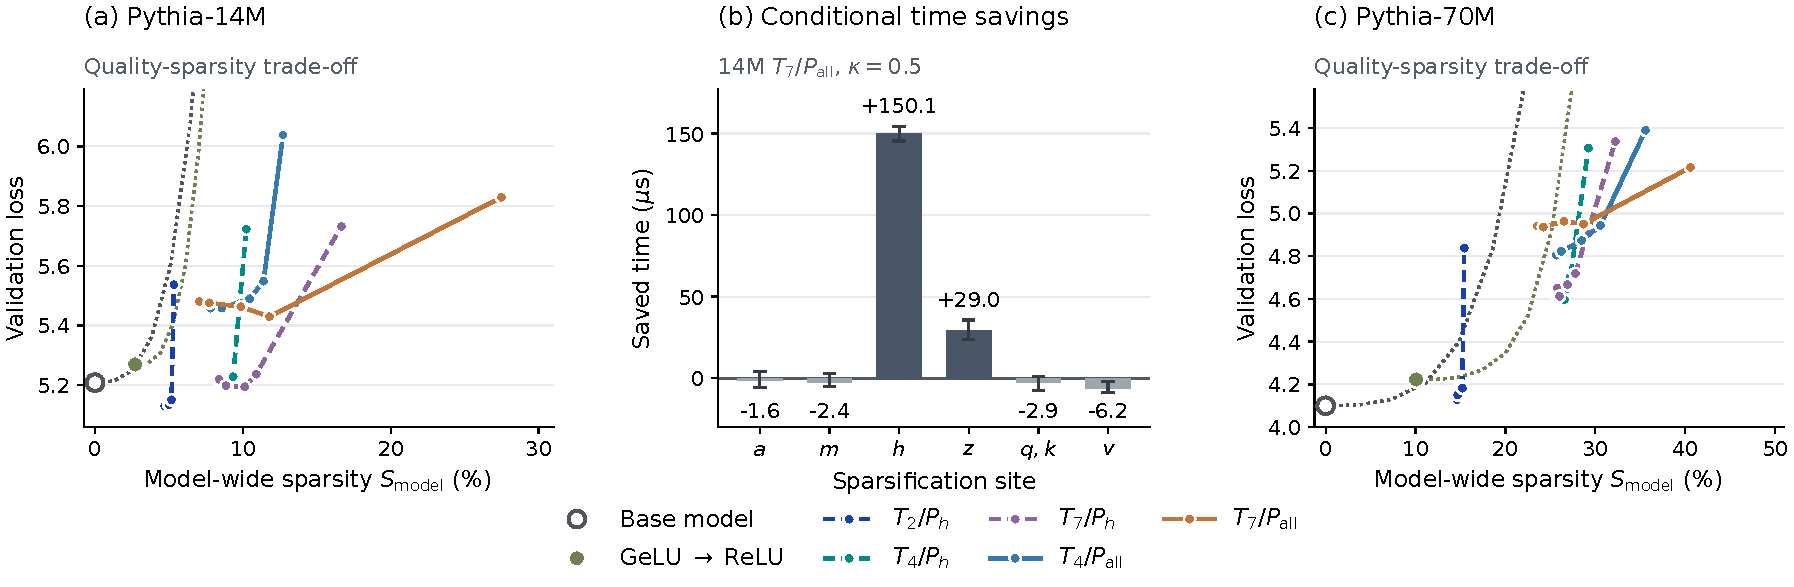
\includegraphics[width=\linewidth]{figures/24-quality-sites-quality.pdf}
% \caption{\textbf{From broad sparsification to targeted execution and scale transfer.}
% \textbf{(a)} Pythia-14M validation loss versus model-wide logical sparsity $\Smodel$ exposes the quality costs of different thresholding and pressure placements.
% \textbf{(b)} Conditional execution ablations on $T_7/P_{\mathrm{all}}$ at $\kappa=0.5$ identify $h$ and $z$ as the profitable skipping sites, motivating the narrower $T_2/P_h$ recipe.
% % Saved time is full-model latency with one skipping path disabled minus latency with all paths enabled; whiskers span all differences between the three process means per mode. These effects are not additive. Timings use BF16 on an RTX~5090, batch one and 2,048 tokens; $q,k$ are ablated jointly.
% \textbf{(c)} Pythia-70M tests the quality--sparsity trade-off at a larger scale: $T_2/P_h$ retains near-baseline quality for $\kappa\leq0.1$, while its most aggressive threshold also incurs a quality cost.
% Panels (a,c) each show 27 trained checkpoints from the seven shared recipes in the legend; curves connect $\kappa=0,.01,.05,.1,.5$. Dotted Base/ReLU curves show post-hoc clipping.
% }
% \label{fig:quality-sparsity-overview}
% \end{figure}

% This mismatch motivates two diagnostic questions: (i) \emph{where does sparsity actually emerge across the network}, and (ii) \emph{where does that sparsity actually save execution time?} Decomposing sparsity across sites and layers reveals a nonlocal response that we call \emph{sparsity spillover}: pressure applied only at the FFN hidden activation $h$ substantially increases sparsity not only at $h$, but also at the unpressured attention-output activation $z$. An independent execution decomposition points to the same locations. Conditional kernel ablations show that the measurable latency savings arise primarily from skipping work at $h$ and $z$, whereas substantial bypass at other sites does not necessarily overcome the overhead required to exploit it. %Thus, the representation-level and execution-level analyses converge on the same pair of sites: $h$ and $z$ are both especially responsive to sparsification and especially profitable for sparse execution.

% % 14M control: Run048 observations/001-causal-hz-latency.md; 07_reduce.py.
% This convergence suggests a narrower intervention, $T_2/P_h$, which applies pressure only at $h$ and thresholds only $h$ and $z$. At 14M, $T_2/P_h$ preserves quality while exposing sparsity at these two sites. At $\kappa=0.1$, exploiting these zeros reduces latency by $12.9\%$ relative to the same implementation with $h,z$ skipping disabled, while preserving the activations and outputs. We then promote $T_2/P_h$ together with the broader $T_4$ and $T_7$ recipes to Pythia-70M. The quality--sparsity ordering transfers: $T_2/P_h$ remains close to the dense model's validation loss while approaching the sparsity directly reachable through $h$ and $z$, while broader recipes attain greater model-wide sparsity at substantially larger quality cost.

% Sparse execution, however, does not transfer automatically. A direct adaptation of the 14M kernel to 70M adds enough overhead to offset much of the additional sparse gains. To profitably explore the 70M sparsity, it is required additional kernel development and optimization. We argue that activation sparsity is an execution co-design problem. A scalar sparsity percentage is insufficient: training must induce zeros at sites and granularities where kernels can avoid expensive memory movement and computation. Controlled intervention and execution ablations reveal that different transformer sites have radically different sparsification and execution value.
% %These results show that activation sparsification should be viewed as a co-design training-and-execution problem: training should induce the properties that inference system can exploit, rather than maximizing a generic sparsity metric and attempting to accelerate the resulting representation afterward.

% %-----------------
% % Transformer blocks expose several candidate activation sites. 

% to study the effects of (i) activation $\ell_1$ pressure ($P$) and (ii) \emph{thresholding} ($T$). While pressure adds a gradient component to induce smaller activation magnitudes, thresholding maps small values into exact zeros. Each one of them can be placed in different activation sites, giving a combinatorial design set of sparse interventions. For each combination of $P$ and $T$, we derive an architecture-dependent maximum achievable sparsity ($\Smax$), measure model-wide attained activation sparsity ($\Smodel$) and evaluate the final inference latency under a specialized sparse kernel. Figure~\ref{fig:quality-sparsity-overview} presents sparsity vs. quality trade-offs and inference latency for Pythia-14M, across $P/T$ combinations and baseline controls.

% % 14M-only main figure, authorized 20 September 2026; copy hash in figures/SOURCES.json.
% % Figure source: analyses/027-2026-09-20-run044-manuscript/02_plot.py
% % Observation: analyses/027-2026-09-20-run044-manuscript/observations/001-run044-integration.md
% % Checkpoint identities and coordinates: analyses/027-2026-09-20-run044-manuscript/data/figure-data.json
% \begin{figure}[!t]
% \centering
% 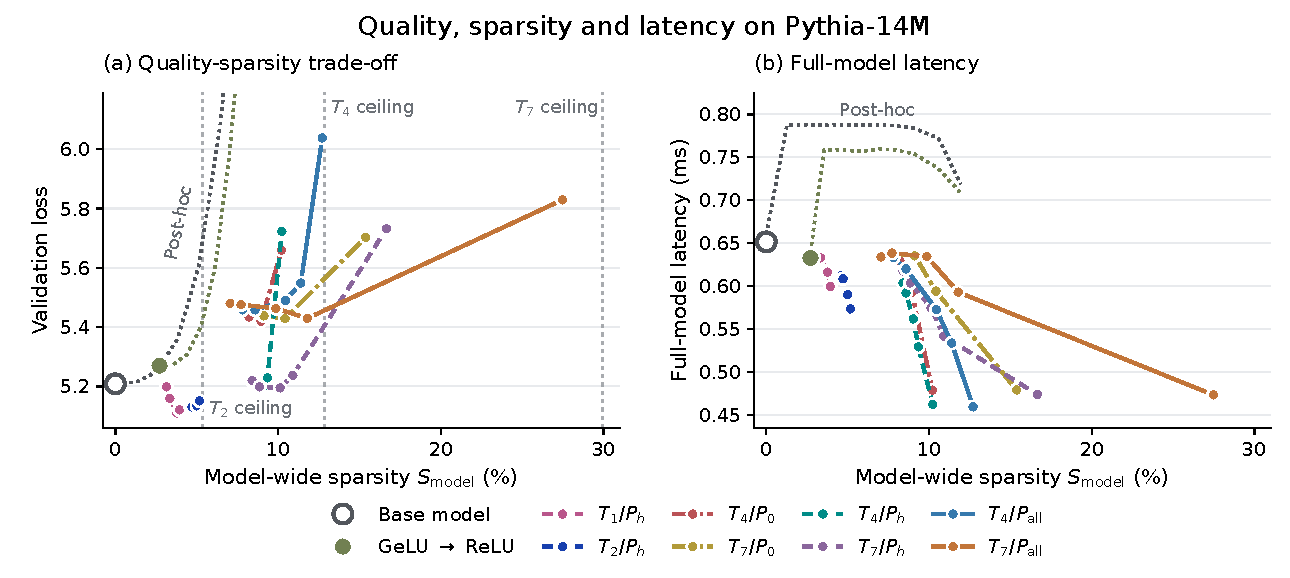
\includegraphics[width=0.9\linewidth]{figures/22-14m-main-quality-sparsity-latency.pdf}
% \caption{\textbf{Quality, sparsity and execution on Pythia-14M.}
% \textbf{(a)} Final validation loss and \textbf{(b)} full-model latency versus $\Smodel$ for 41 checkpoints spanning the Base/ReLU controls and the $T/P$ intervention grid. Curves connect separately trained settings over $\lambda=.05,.1,.5,1$ for $T_1/P_h$ and $\kappa=0,.01,.05,.1,.5$ otherwise. Dotted curves in (a) show post-hoc clipping of the Base/ReLU controls; vertical dotted lines mark analytic sparsity ceilings. Latencies use an RTX~5090, batch one, and 2,048-token sequences.
% }
% \label{fig:quality-sparsity-overview}
% \end{figure}

% % Editorial revision: reviews/2026-09-20-introduction-abstract/README.md (surgical revision).
% % Evidence: Analysis024 observations 015, 028, 034, 041; Analysis021 pressure-scope O016.
% Across 41 14M-parameter and 27 70M-parameter training and evaluation runs, we identify several insights.
% First, \textbf{the $T/P$ train-time interventions extend the attainable sparsity range relative to post-hoc clipping}, approaching the architectural ceiling for the more aggressive recipes, but at a cost in quality (Figures~\ref{fig:quality-sparsity-overview} and~\ref{fig:70m-quality-latency}).
% Second, \textbf{sparsity and speedup increase together within recipes}, but a larger $\Smodel$ does not directly translate into a larger speedup. Lower latency depends on the location and structure of zeros, and whether the kernel can exploit them. At 14M, most speedup gains come from skipped computation at FFN-hidden ($h$) and Post-attention projection ($z$) sites (Table~\ref{tab:kernel-mechanisms}).
% % Scale-check evidence: Run042 observation 001; Analysis028 observations/001-matched-70m-grid.md.
% Third, \textbf{sparsity remains exploitable across the tested scales}: skipping computations can reduce latency at both 14M and 70M, but the 14M implementation did not transfer efficiently; 70M required an additional kernel optimization step (Appendix~\ref{app:kernel-transfer}).
% Fourth, \textbf{local pressure at $h$ provides a more favorable balance between quality, sparsity and latency than global pressure}. At 14M, pressure at $h$ and thresholding at $h,z$ with $\kappa\leq0.1$ provide additional speedup with almost no quality degradation (Figure~\ref{fig:quality-sparsity-overview}).
% Finally, \textbf{local pressure can induce global changes in sparsity}. Pressure at $h$ increases sparsity at $z$, even if it receives no direct pressure (Figure~\ref{fig:pressure-layer-sparsity}). This is evidence that some sites are more succeptible to sparsification. 
% Taken together, these results indicate that activation sparsification should not be treated as an isolated training objective: interventions and deployment kernels must be co-designed so that the induced sparsity is both high and structurally exploitable at inference time.
